%!TEX root = main.tex


In this chapter the architecture of the system will be described. The 4+1 model will be used. We will be describing  the logical view, the physical view, the process view and the data view. 
The logical view shows the functional decomposition of the architecture into components.
the process view shows behavioral aspects of the system, the data flow view defines the data, the relation
between data entities, how the data flows through the system and the measures to ensure reliability and
performance. The physical view shows the physical entities and storage units as well as the deployment
scenario.

\section{Logical View}
This view shows the connections between structural elements, key abstractions and mechanisms that are used within SFM. At first, an overview of the components is provided. The main components of the system will be displayed in terms of layers. Next, the main components are decomposed a in term of responsibilities and interfaces.

\subsection{Primary presentation}
In order to design the software architecture of \ac{ET}, the layers pattern is used. This pattern is best suitable for the system since it gives the opportunity to abstract layers from one another, which increases the availability of the system by modularizing the components. The modularization of the components increases also the scalability and the performance of the system. 
The system has been structured according to the three-layers approach. The three main components: Mobile app, Beacon Interface and the Local Storage, and Central storage and Payment system can be seen in the figure below. 


\begin{figure}[H]
  \centering
  \includegraphics[width=\textwidth]{Pictures/arch.png}
  \caption{Overview of the System}
  \label{fig:system}
\end{figure}


\textbf{Mobile app} is the main component of our system. It will be available for download for the users and it will provide a personalized and unique account for the passengers. They can use this account to login and pay for their ticket, every time they use the trains. This layer will also enable a bluetooth connection with the beacon cart. The data collected from this layer is then sent to the other layers. 

\textbf{Beacon Interface and Local storage} This layer creates a connection with the mobile app layer. Its components are the local storage, where the data gathered from the mobile app will be stored, and the beacon interface which establishes the bluetooth connection with the mobile.

\textbf{Central Storage and Payment system} The database and the Beacon Interface are included in this layer. The data that is provided from the Mobile app layer, will be stored in the central database after the mobile phone has connected to the beacon. The calculation of the ticket fees is also done in this layer through the computational center.

\begin{figure}[H]
  \centering
  \includegraphics[width=\textwidth]{Pictures/logical.png}
  \caption{Logical View}
  \label{fig:logical}
\end{figure}

\section{Process View}
This section describes the main processes performed by the system following some of the main use cases presented in chapter \ref{chp:usecases}. The following system sequence diagrams will help detail every such process by displaying the main information flows between different actors and system components in a chronological manner.

\begin{figure}[H]
	\centering
	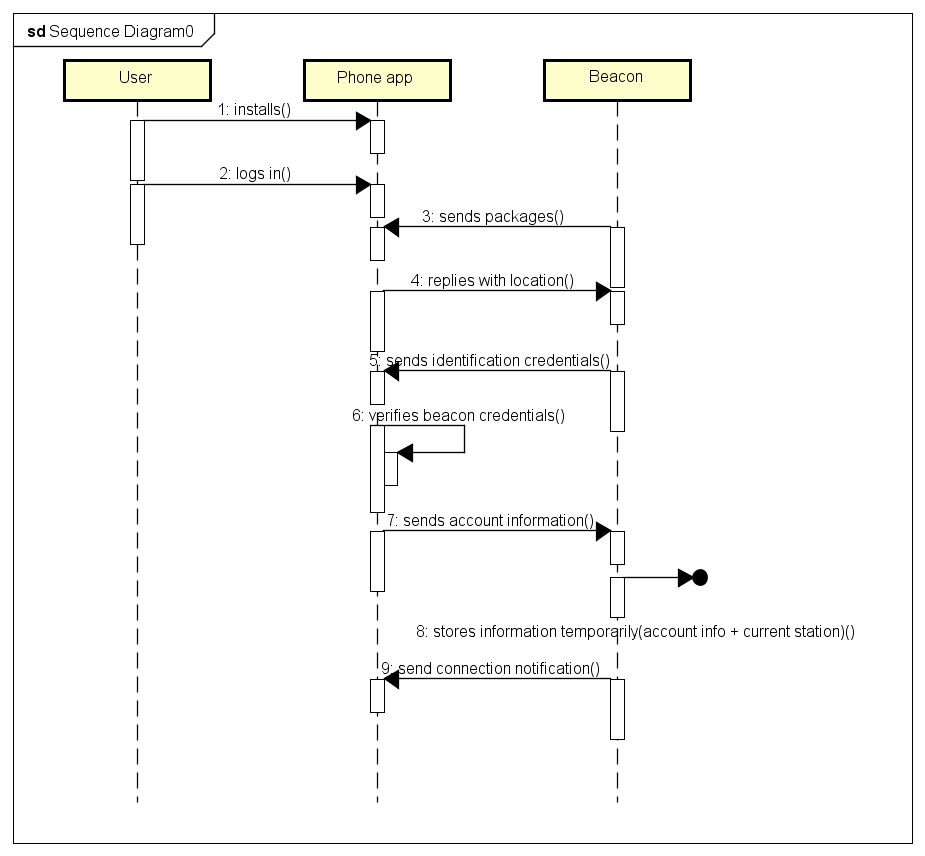
\includegraphics[width=\textwidth]{Pictures/seq_diagram_uc1.png}
	\caption{System sequence diagram- use case 1(Connect phone to beacon)}
	\label{fig:seqDiagram1}
\end{figure}
Figure \ref{fig:seqDiagram1} is a direct mapping of use case 1(connect phone to beacon).

\begin{figure}[H]
	\centering
	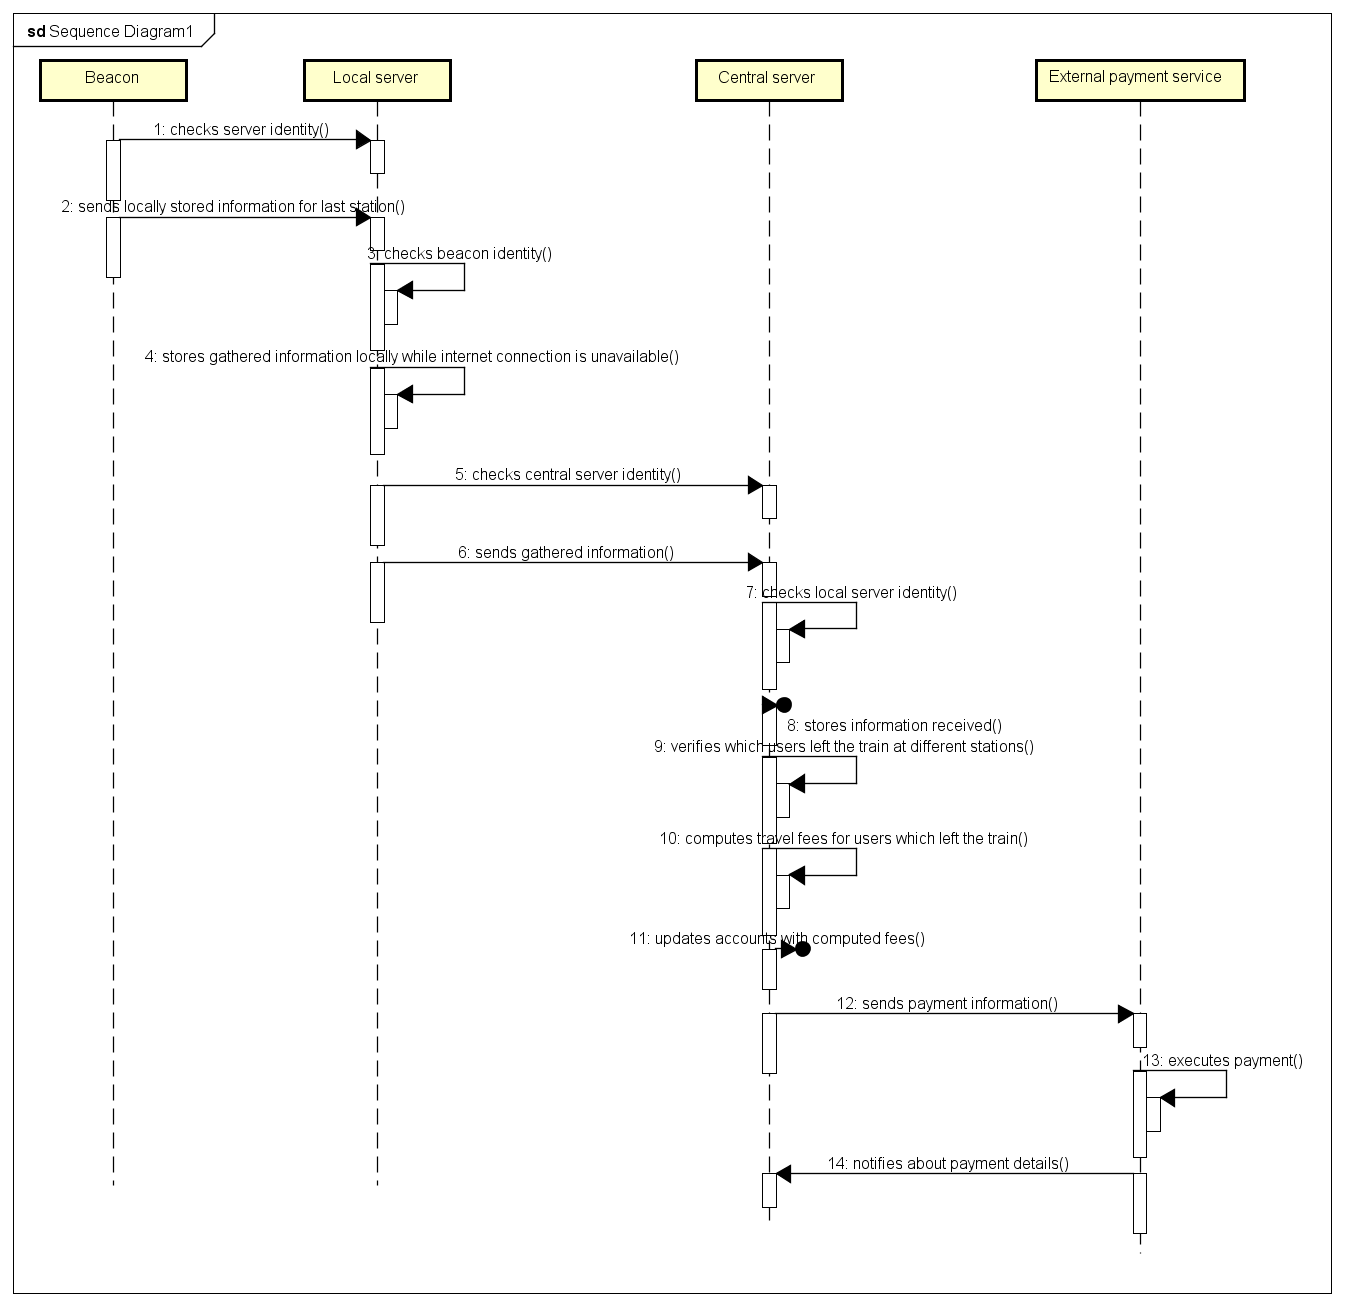
\includegraphics[width=\textwidth]{Pictures/seq_diagram_payment.png}
	\caption{System sequence diagram- payment}
	\label{fig:seqDiagram2}
\end{figure}
Figure \ref{fig:seqDiagram2} displays the information flow corresponding to use cases "Disconnect from beacon" "Calculate travel fee" and "Make payment". For this process, the system uses a third party payment service.

\begin{figure}[H]
	\centering
	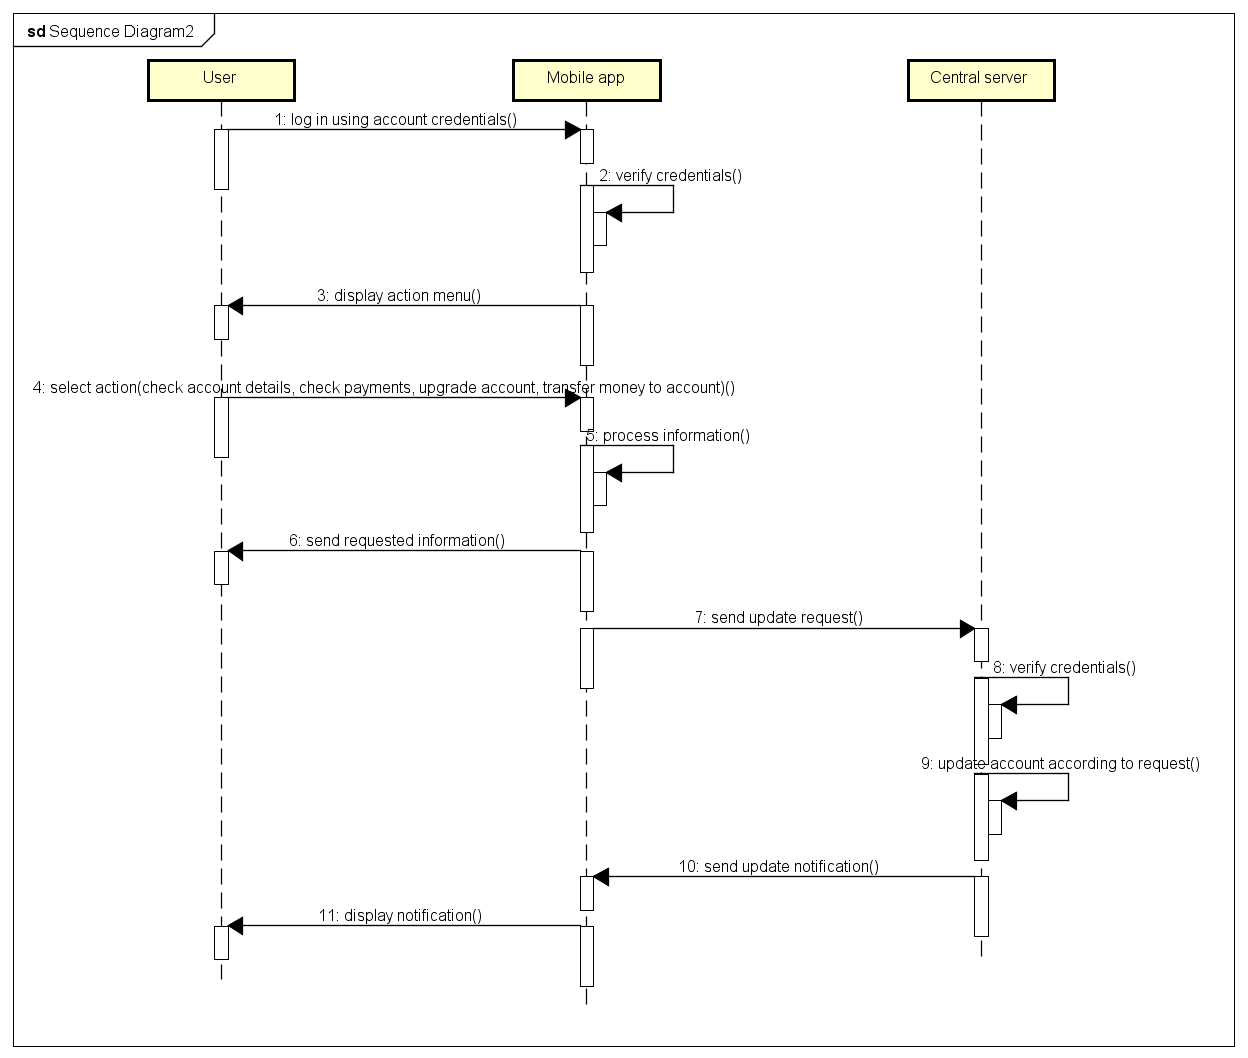
\includegraphics[width=\textwidth]{Pictures/seq_diagram_checkAccount.png}
	\caption{System sequence diagram- Check account details}
	\label{fig:seqDiagram3}
\end{figure}
Figure \ref{fig:seqDiagram3} displays the information flow related to use cases "Register through application", "Check account balance" and "Login through application". This process describes the general outline for different actions the user can perform using the mobile application.


\begin{figure}[H]
	\centering
	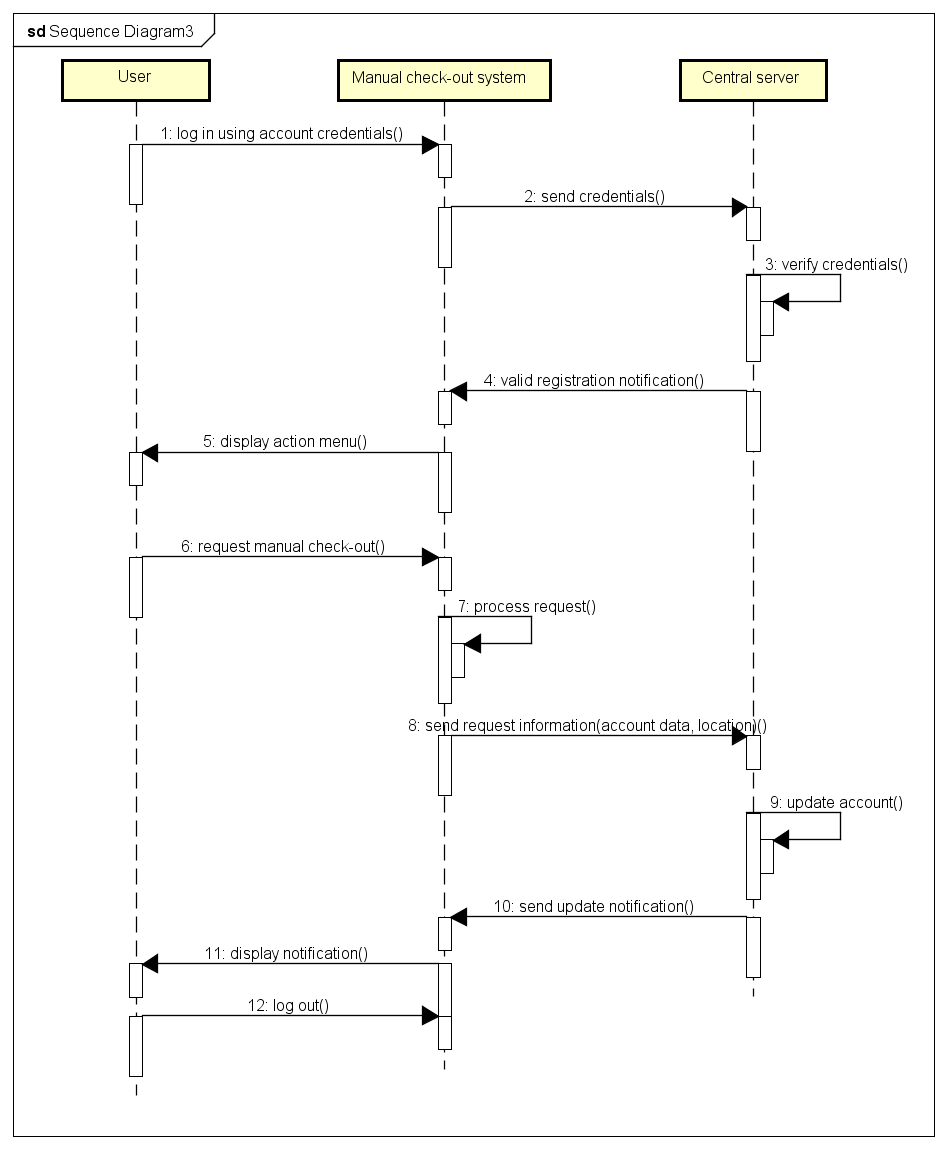
\includegraphics[width=\textwidth]{Pictures/seq_diagram_manualCheckOut.png}
	\caption{System sequence diagram- Manual checkout}
	\label{fig:seqDiagram4}
\end{figure}
Figure \ref{fig:seqDiagram4} shows the main information flow corresponding to the use case "Manually sign out from journey". This use case was designed as an alternative to the main "Disconnect from beacon" use case which will give users the possibility to manually check out at a particular train station in case of the phone to beacon connection not being available.

%\section{Data View}-- what is data view?
%\section{Physical View}